%\documentstyle[epsf,twocolumn]{jarticle}       %LaTeX2.09仕様
\documentclass{jarticle}     %pLaTeX2e仕様

%\usepackage[backend=bibtex, style=numeric]{biblatex}
%\addbibresource{sankou.bib}
%%%%%%%%%%%%%%%%%%%%%%%%%%%%%%%%%%%%%%%%%%%%%%%%%%%%%%%%%%%%%%
%%
%%  基本 バージョン
%%
%%%%%%%%%%%%%%%%%%%%%%%%%%%%%%%%%%%%%%%%%%%%%%%%%%%%%%%%%%%%%%%%
\setlength{\topmargin}{-45pt}
%\setlength{\oddsidemargin}{0cm}
\setlength{\oddsidemargin}{-7.5mm}
%\setlength{\evensidemargin}{0cm}
\setlength{\textheight}{24.1cm}
%setlength{\textheight}{25cm}
\setlength{\textwidth}{17.4cm}
%\setlength{\textwidth}{172mm}
\setlength{\columnsep}{11mm}

\setlength{\intextsep}{8pt}
\setlength{\textfloatsep}{8pt}
\setlength{\floatsep}{1pt}

\kanjiskip=.07zw plus.5pt minus.5pt



%【節がかわるごとに(1.1)(1.2) …(2.1)(2.2)と数式番号をつけるとき】
%\makeatletter
%\renewcommand{\theequation}{%
%\thesection.\arabic{equation}} %\@addtoreset{equation}{section}
%\makeatother

%\renewcommand{\arraystretch}{0.95} 行間の設定

\usepackage[dvipdfmx]{graphicx}   %pLaTeX2e仕様(\documentstyle ->\documentclass)
\usepackage{scalefnt}
\usepackage{bm}
\usepackage{here}
\usepackage{url}
\usepackage{amsmath}
\usepackage{amsfonts}
\usepackage[subrefformat=parens]{subcaption}
\captionsetup{compatibility=false}
%%%%%%%%%%%%%%%%%%%%%%%%%%%%%%%%%%%%%%%%%%%%%%%%%%%%%%%%
\usepackage{comment}
\usepackage{subcaption}
\usepackage{multirow}
\usepackage{nidanfloat}
\usepackage[dvipdfmx]{hyperref}

\usepackage[normalem]{ulem}
\useunder{\uline}{\ul}{}

\begin{document}

\twocolumn[
\noindent
\hspace{1em}

令和2年6月10日(水) ゼミ資料
\hfill
\ \ B4 高山 裕成

\vspace{2mm}
\hrule
\begin{center}
{\Large  進捗報告}
\end{center}
\hrule
\vspace{3mm}
]


% \footnotesize

\section{進捗}
ipsj 支部の発表パワポ

\section{4 コマ漫画ストーリーデータセット拡張のための手法提案}
\subsection{想定}
\begin{itemize}
  \item Google Form または
  \item 自作ツール
\end{itemize}
\subsubsection{事前処理}
すべてのコマに含まれるフキダシ内を白抜きにし, 番号を割り振る.

\subsubsection{仕様}
\begin{itemize}
  \item エディターには固有の ID が与えられる
  \item エディターには登場人物の名前を独自に決めてもらう
  \item 各タッチについて 4 コマ内のセリフを考えてもらい, 感情ラベルも付けてもらう
  \item 4 コマ内での話の一貫性を保ってもらう
  \item フキダシの大きさとセリフの量の制限については未確定
\end{itemize}

感情ラベルは本データセットの仕様に合わせる.

\subsubsection{Google Form}

\begin{figure*}[!bth]
  \begin{center}
    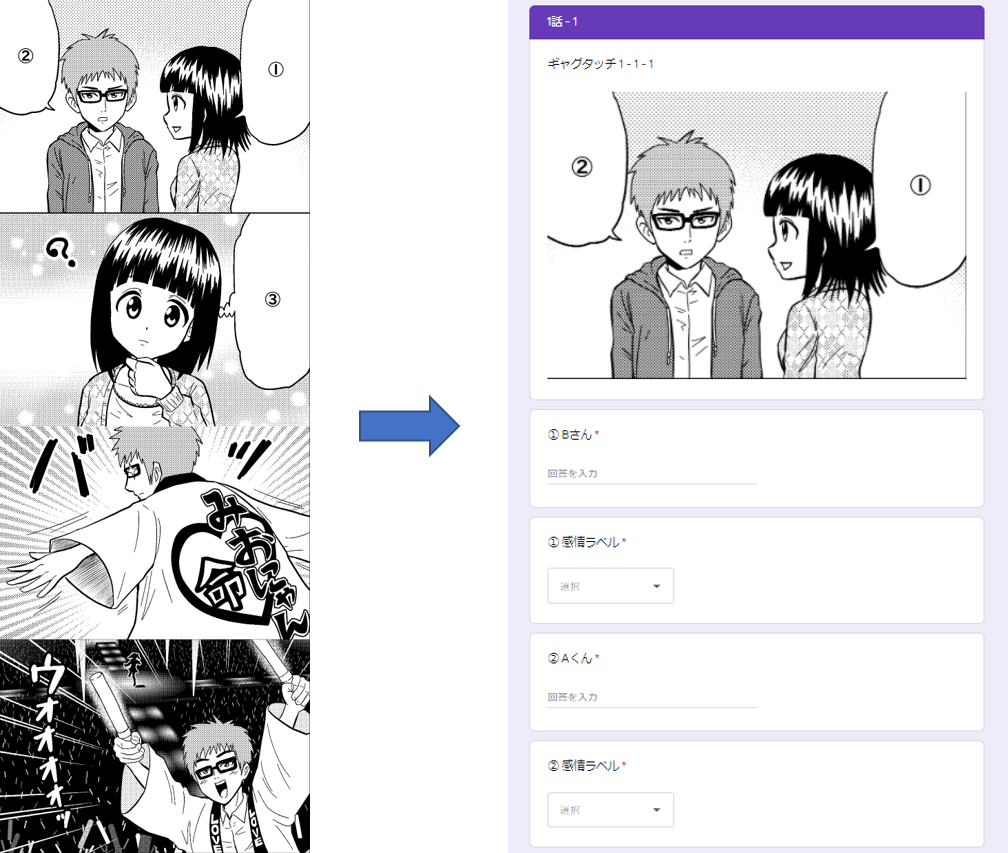
\includegraphics[scale=0.7]{form.png}
    \caption{Google Form 概要} %タイトルをつける
    \label{fig:form} %ラベルをつけ図の参照を可能にする
  \end{center}
\end{figure*}

\begin{itemize}
  \item まず, 4 コマ全体を見せる
  \item 1 コマずつ, 含まれるセリフについてラベルとともに決めてもらう
\end{itemize}

メリット

\begin{itemize}
  \item 特に何も考えなくても取り敢えず回答を集めることが可能
\end{itemize}

デメリット

\begin{itemize}
  \item 操作が煩雑・編集の難しさ
  \item フォーム作成を全手動でやるのは面倒 (GAS の勉強が必要)
  \item 回答を整形しなおさないといけない
  \item データセットの権利関係が分からない
  \item コマ画像は別窓で開いてもらう方がいいかも
\end{itemize}

\subsubsection{自作ツール}

\begin{figure*}[!tbh]
  \begin{center}
    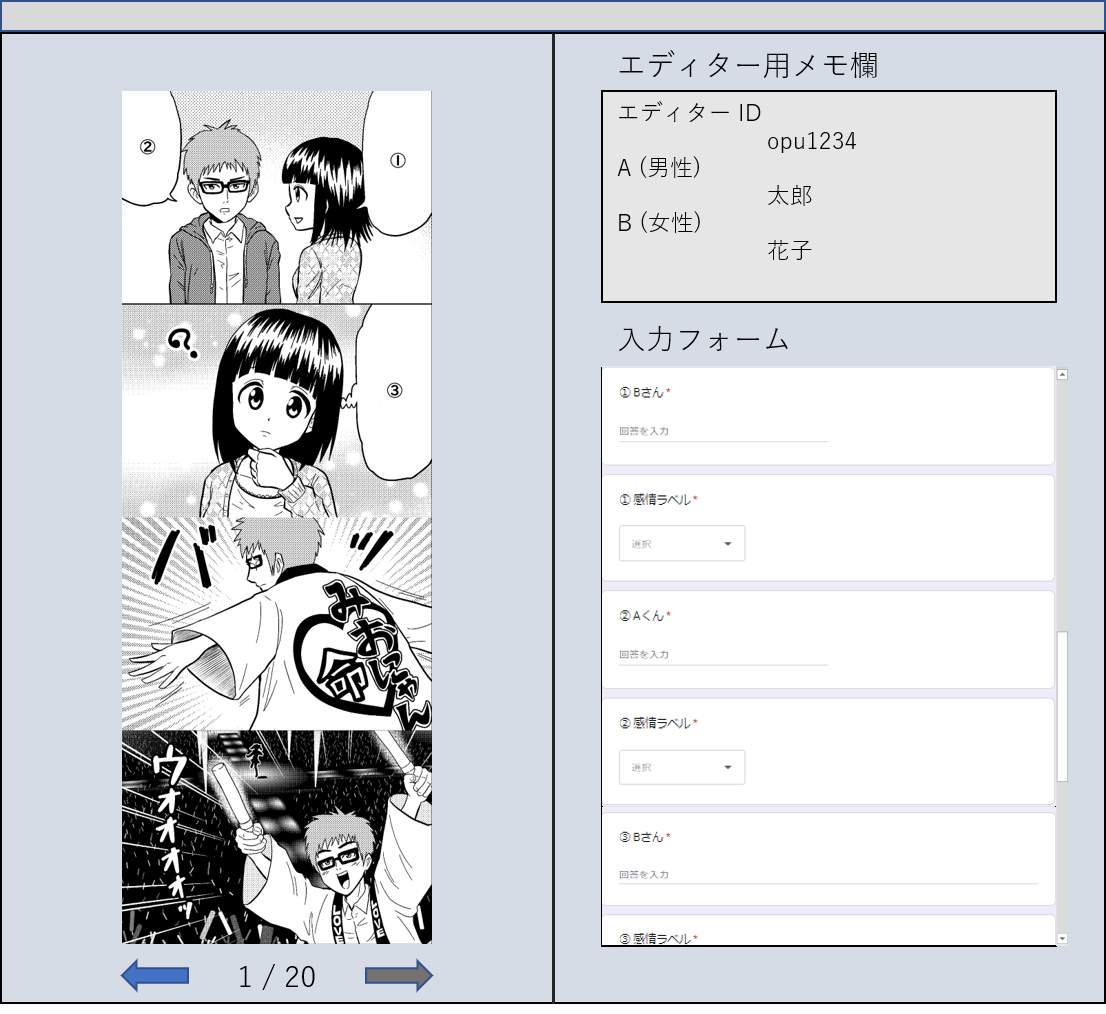
\includegraphics[scale=0.7]{tool.png}
    \caption{自作ツール 概要} %タイトルをつける
    \label{fig:tool} %ラベルをつけ図の参照を可能にする
  \end{center}
\end{figure*}

\begin{itemize}
  \item GUI アプリケーション
  \item csv ファイルに自動保存
\end{itemize}

メリット

\begin{itemize}
  \item 4 コマ全体を見ながら入力できる
  \item アプリ上ですべてのタッチ・コマに対して編集可能
  \item 操作・編集が楽
\end{itemize}

デメリット

\begin{itemize}
  \item 開発 (何を使えばいいかわからない. PyQt, Tkinter, kivy ...)
\end{itemize}

\section{今後の予定}
\begin{itemize}
  \item ipsj 支部発表本番
  \item セリフから話者の推定
\end{itemize}

\bibliographystyle{unsrt}
\bibliography{sankou}


\end{document}
